\chapter{Online Password Cracking}

Questo tipo di attacco si basa su un utente malintenzionato che proverà ad indovinare le credenziali di un utente per la pagina di accesso di un'applicazione web; per un server SSH o Telnet; o per un servizio di rete come LDAP (Lightweight Directory Access Protocol), uno dei protocolli di posta (SMTP, POP3 o IMAP), FTP o uno dei tanti altri.

Gli attacchi di Brute Force online, a differenza di quella offline, vanno incontro a più problematiche, come alla larghezza di banda della reta, blocco dell'account e rilevamento nei registri.

Per gli attacchi online sono più adatti i Dictionary Attack che fanno uso di dizionari di piccole dimensioni e mirati piuttosto che all'uso di Brute Force.

Il vantaggio principale di eseguire un Online Password Cracking è che un utente malintenzionato non ha bisogno di privilegi speciali per avviare l'attacco. Il computer attaccato fornisce alcuni servizi ai suoi utenti legittimi e un attacco di cracking delle password online riuscito consente all'attaccante di avere gli stessi privilegi dell'utente le cui credenziali sono state indovinate.

In secondo luogo, esiste un'ampia varietà di protocolli che possono essere attaccati. Qualsiasi protocollo di rete che accetta login e password può essere attaccato con Online Password Cracking.

Infine, Online Password Cracking può essere avviato letteralmente da qualsiasi parte del mondo su Internet, da qualsiasi computer che ha accesso alla rete al servizio attaccato.

\section{Strumenti}

Nella rete si possono trovare infiniti tool che permettono di eseguire questo tipo di attacco, ora ne vedremo i più famosi.

\subsection{Hydra}

Hydra \cite{hydra} è un cracker di accesso in parallelo che supporta numerosi protocolli per attaccare. È molto veloce e flessibile e i nuovi moduli sono facili da aggiungere. Questo strumento consente a ricercatori e consulenti di sicurezza di mostrare quanto sarebbe facile ottenere l'accesso non autorizzato a un sistema da remoto.

Supporta innumerevoli servizi web : Cisco AAA,s Cisco auth, Cisco enable, CVS, FTP, HTTP(S)-FORM-GET, HTTP(S)-FORM-POST, HTTP(S)-GET, HTTP(S)-HEAD, HTTP- Proxy, ICQ, IMAP, IRC, LDAP, MS-SQL, MySQL, NNTP, Oracle Listener, Oracle SID, PC-Anywhere, PC-NFS, POP3, PostgreSQL, RDP, Rexec, Rlogin, Rsh, SIP, SMB(NT) , SMTP, SMTP Enum, SNMP v1+v2+v3, SOCKS5, SSH (v1 e v2), SSHKEY, Subversion, Teamspeak (TS2), Telnet, VMware-Auth, VNC e XMPP.

La sintassi per eseguire un attacco con Hydra è la seguente :

\begin{lstlisting}[ caption={Hydra esempio}, style=javaScriptCode]
    root@kali:~# hydra -l user -P passlist.txt ftp://192.168.0.1
    root@kali:~# hydra -L userlist.txt -p defaultpw imap://192.168.0.1/PLAIN
    root@kali:~# hydra -C defaults.txt -6 pop3s://[2001:db8::1]:143/TLS:DIGEST-MD5
    root@kali:~# hydra -l admin -p password ftp://[192.168.0.0/24]/
    root@kali:~# hydra -L logins.txt -P pws.txt -M targets.txt ssh
\end{lstlisting}

In questo esempio di eseguirà un semplice attacco, andando a testare lo user "root" e la password "toor" sull'indirizzo 127.0.0.1 utilizzando il protocollo ssh.

In Hydra abbiamo molte opzioni che se possono applicare per migliorare i nostri attacchi, come :
\begin{itemize}
    \item \textbf{-l} login con un nome specifico (passato dopo il comando)
    \item \textbf{-L} login testando tutti gli utenti inserite all'interno di un file 
    \item \textbf{-p} prova una password specifica (passato dopo il comando)
    \item \textbf{-P} prova tutte le password presenti in un file passato
    \item \textbf{-s} viene utilizzato per specificare una porta in cui eseguire l'attacco 
    \item \textbf{-x} utilizzato per la generazione delle password per eseguire il Brute Force, dopo il comando gli si passa MIN:MAX:CHARSET
    \item \textbf{-y} disabilita l'uso di simboli per ;a generazione di password nel Brute Force
\end{itemize}

Vediamo insieme un attacco con Hydra 

\begin{figure}[htpb!]
    \centering
    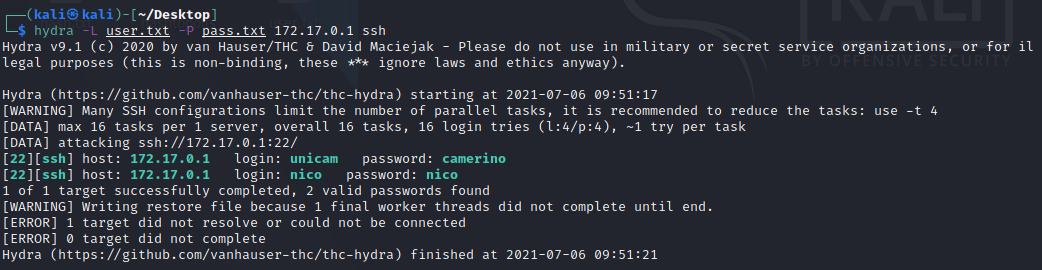
\includegraphics[width=\linewidth]{Immagini/5/hydra.png}
    \caption{Hydra esempio}
    \label{fig:Hydra example}
\end{figure}

\begin{lstlisting}[ caption={Hydra code example}, style=javaScriptCode]
    root@kali:~# hydra -L user.txt -P pass.txt 172.17.0.1 ssh
\end{lstlisting}

In questo attacco andiamo ad utilizzare una lista di utenti e una lista di password per eseguire il Brute Force, infine andremo a specificare l'indirizzo su cui eseguire il Brute Force e su quale servizio.

Possiamo vedere che si è trovata la corrispondenza per due utenti (nico e unicam), con le seguenti password (nico e camerino). 
\newpage

\subsection{WpScan}

WPScan\cite{wpscan} è un web scanner creato per analizzare e cercare falle di sicurezza all’interno della piattaforma di blogging WordPress. Il tool WPScan è in grado di testare un sito che adotta un WordPress e controllare la presenza di vulnerabilità che devono essere sistemate, purtroppo molte volte anche zero day.

Una particolarità di questo tool è il fatto di poter eseguire un attacco Brute Force tramite l'utilizzo di dizionari per il login nell'area "admin" di questi siti creati in wordpress.

\begin{figure}[htpb!]
    \centering
    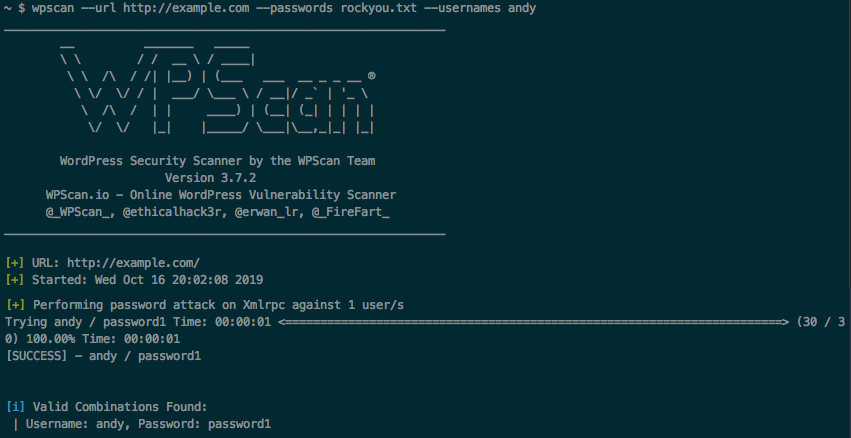
\includegraphics[width=\linewidth]{Immagini/5/wpscan_example.png}
    \caption{WpScan example\cite{wpscan_example}}
    \label{fig:WpScan example}
\end{figure}

\begin{lstlisting}[ caption={WpScan code example}, style=javaScriptCode]
    root@kali:~# wpscan --url http://example.com --password rockyou.txt --usernames andy
\end{lstlisting}

Una volta eseguito l'attacco verrà mostrato a video le credenziali di accesso, come nell'esempio precedentemente riportato.

Per testare più utenti, basta aggiungere dopo il comando \textbf{--usernames}, i nomi dei vari utenti da testare, separati da una virgola.

\newpage


\subsection{GoBuster}

GoBuster\cite{gobuster} è un tool per il Brute Force scritto in Go, questo linguaggio permette di avere prestazioni altamente elevate a differenza di altri Strumenti che possiamo trovare che risultano molto più lenti (per esempio Dirbuster, DirSearch, DIRB). Lo scopo di questo tool è quello di eseguire il Brute Force per scoprire le directory di un sito, sottodomini DNS e nomi di host virtuali sui server web.

\begin{figure}[htpb!]
    \centering
    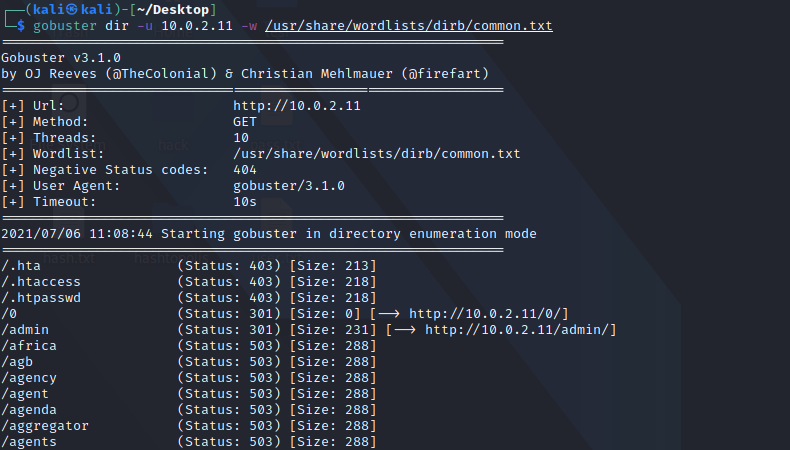
\includegraphics[width=\linewidth]{Immagini/5/gobuster.png}
    \caption{gobuster example}
    \label{fig:gobuster example}
\end{figure}

La sintassi di questo tool è basata sull'utilizzo dei seguenti parametri :
\begin{itemize}
    \item \textbf{dir} viene utilizzato per indicare la ricerca di directory
    \item \textbf{dns} viene utilizzato per indica la ricerca dei sottodomini DNS
    \item \textbf{vhost} viene utilizzato per indicare la ricerca dei nomi dei host virtuali
    \item \textbf{-u} opzione  utilizzata per specificare l'url sul quale eseguire l'attacco
    \item \textbf{-z} opzione utilizzata per nascondere il progresso dell'attacco
    \item \textbf{-o} opzione utilizzata per specificare un file per l'output 
    \item \textbf{-t} opzione utilizzata per indicare il numero di thread da utilizzare 
    \item \textbf{-w} opzione utilizzata per indicare la wordlist per l'attacco
\end{itemize}

\begin{lstlisting}[ caption={GoBuster code example}, style=javaScriptCode]
    root@kali:~# gobuster dir -u https://www.google.it -w /usr/common.txt -o prova.txt
\end{lstlisting}

\label{chap:conc}

